\documentclass[a4paper,german,12pt]{scrartcl}
\usepackage[T1]{fontenc}
\usepackage[utf8]{inputenc}
\usepackage{babel}
\usepackage{tikz}
\usepackage{geometry}
\usepackage{amsmath}
\usepackage{amssymb}
\usepackage{float}
\usepackage{enumerate}
\usepackage{graphicx}
%\usepackage{wrapfig}
\usepackage[thinspace,thinqspace,squaren,textstyle]{SIunits}
\restylefloat{table}
\geometry{a4paper, top=15mm, left=20mm, right=40mm, bottom=20mm, headsep=10mm, footskip=12mm}
\linespread{1.5}
\setlength\parindent{0pt}
\begin{document}
\begin{center}
\bfseries % Fettdruck einschalten
\sffamily % Serifenlose Schrift
\vspace{-40pt}
Analysis II, Wintersemester 2013/2013, 1. Übungsblatt

Luis Herrmann, Markus Fenske, Tutor: Earl Campbell
\vspace{-10pt}
\end{center}

\section*{Exercise 1}

\begin{enumerate}[(a)]
\item The energy of a photon is given by:
\begin{equation*}
E=hf=\frac{hc}{\lambda}
\end{equation*}

The eV is defined as:
\begin{equation*}
1eV=1,6022\cdot 10^{-19}J
\end{equation*}

Using these formulae, we obtain the following values:

\begin{enumerate}
\item $E_1=\frac{6,6261\cdot 10^-34 Js}{299792458ms^{-1}\cdot 313,2\cdot 10^{-9}m}\approx 6,3462\cdot 10^{-19}J\approx3,9609eV$\\
Spectre: Visible (V)
\item $E_2=\frac{6,6261\cdot 10^-34 Js}{299792458ms^{-1}\cdot 546,0\cdot 10^{-9}m}\approx 3,6403\cdot 10^{-19}J\approx2,2721eV$\\
Spectre: Visible (V)
\item $E_3=\frac{6,6261\cdot 10^-34 Js}{299792458ms^{-1}\cdot 140,2\cdot 10^{-9}m}\approx 0,1418\cdot 10^{-19}J\approx8,8485eV$\\
Spectre: Ultraviolett (UV)
\item $E_4=\frac{1,6261\cdot 10^-34 Js}{299792458ms^{-1}\cdot 1207,2\cdot 10^{-9}m}\approx 1,6565\cdot 10^{-19}J\approx1,0276eV$\\
Spectre: Infrared (IR)
\end{enumerate}


\begin{equation*}
P=|S|A=IA \Rightarrow E=IAt
\end{equation*}

\item $I=10^{-10}Wm^{-2} \quad \lambda=560nm \quad A=0,5cm^2$

The energy of the electromagnetic wave being quantized, we have to impose:
\begin{center}
$nE_0=E$\\
$\Leftrightarrow \frac{nhc}{\lambda}=IAt$\\
$\Leftrightarrow \frac{n}{t}=\frac{IA\lambda}{hc}$
\begin{equation*}
\Leftrightarrow \frac{n}{t}=\frac{10^{-10}Wm^{-2}\cdot 5\cdot10^{-5}m^2\cdot 560\cdot 10^{-9}m}{6,6261\cdot 10^{-34}Js \cdot 299792458ms^{-1}}=14.095s^{-1}
\end{equation*}
\end{center}

The emission rate is roughly $14,1k$ photons per second.

\end{enumerate}

\section*{Exercise 2}

\begin{enumerate}[(a)]

\item
Planck's radiation formula is given as:
\begin{equation*}
w_\nu = \frac{8\pi}{c^3}\nu^3 \frac{h}{e^{\beta h\nu}-1}, \quad \quad \beta=\frac{1}{k_BT}
\end{equation*}

To find out the extremal values of $w_\nu(\nu)$, we set:
\begin{equation*}
\frac{\partial w_\nu}{\partial \nu}\overset{!}{=}0
\end{equation*}

The derivative of $w_\nu$ being:
\begin{align*}
\frac{\partial w_\nu}{\partial \nu}=\frac{8\pi}{c^3}\cdot 3\nu^2 \cdot \frac{h}{e^{\beta h\nu}-1}+\frac{8\pi}{c^3}\cdot\nu^3\frac{-\beta h^2 e^{\beta h \nu}}{e^{\beta h \nu}-1} \\
=\frac{8\pi}{c^3 \nu^2}\nu^2\frac{h}{e^{\beta h \nu} -1}\left(3-\frac{\beta h e^{\beta h \nu}}{e^{\beta h \nu}}-1\right)
\end{align*}

This delivers two distinct solutions:
\begin{equation*}
\underbrace{\frac{8\pi}{c^3}\nu^2\frac{h}{e^{\beta h \nu} -1}}_{(1)}\cdot \underbrace{\left(3-\frac{\beta h e^{\beta h \nu}}{e^{\beta h \nu}-1}\right)}_{(2)}\overset{!}{=}0
\end{equation*}

\begin{center}
\begin{tabular}{ll}
$\frac{8\pi}{c^3}\nu^2\frac{h}{e^{\beta h \nu} -1}=0$ & \quad \quad $3-\frac{\beta h e^{\beta h \nu}}{e^{\beta h \nu}-1}=0$\\
$\nu=0$  & \quad \quad $3\left(e^{\beta h \nu} -1\right)+\beta h e^{\beta h \nu}=0$\\
& \quad \quad $\frac{3}{e^{\beta h \nu}}=3-\beta h \nu$\\
& \quad \quad $\beta h \nu = 3\left(1-e^{-\beta h \nu}\right)$
\end{tabular}
\end{center}

Let $x=\beta h \nu$:
\begin{align*}
x=3\left(1-e^{-x}\right)\\
\Leftrightarrow x=2,8215\\
\Rightarrow \nu=\frac{2,8215}{\beta h}
\end{align*}

Needless to say, roughly knowing the shape of the function's graph and applying inutitive logic, we can immediately exclude the function having a local maximum at $\nu=0$, where, in fact, we will obtain a local (and global) minimum.\\
 Thus, we are left with one single local and global maximum, namely at:

\begin{equation*}
\nu=\frac{2,8215}{\beta h}=\frac{2,8215k_BT}{h}
\end{equation*}\\

\item Using the previously derived formula for the maximum of radiation density, we get:
\begin{equation*}
\nu=\frac{2,8215\cdot 1,3806 \cdot 10^{-23}JK^{-1}\cdot 5800K}{6,6261\cdot 10^{-34}Js}\approx 3,4098\cdot 10^{14}s^{-1}
\end{equation*}

The spectral energy density has its maximum at a frequency of approximately 341THz.

\item $r=0,005cm\\
 (1)T=2500K \quad \rho(T)=2,5\cdot 10^{-4}\Omega cm\\ (2)T_0=295,15K \quad T=2500K \quad \rho(T_0)=2,5\cdot 10^{-4}\Omega cm$\\

For this calculus, the conductor is to be regarded as an ideal black body. This being the case, we can determine the radiation power using the Stefan-Boltzmann law:
\begin{equation*}
P_{em}=\sigma A T^4, \quad A=2\pi r l
\end{equation*}
A being the radiation surface, which in this case is the surface of the cylindrical conductor with radius $r$ and length $l$ minus the base areas.

The electric power of the wire is given by:
\begin{equation*}
P_{el}=RI^2
\end{equation*}

As it is not specified whether the given specific resistance refers to room temperature or to the given temperature of $T=2500K$, I will do the calculus for both cases.\\

For the first case, the resistance is quite simply:
\begin{equation*}
R=\rho\frac{l}{A_r}, \quad A_r=\pi r^2
\end{equation*}
$A_{r}$ being the cross-section area of the cylindrical conductor.
For the second case:
\begin{equation*}
R=\rho(T)\frac{l}{A_{r}}=\rho(T_0)(1+\alpha(T-T_0))\frac{l}{A_{r}}
\end{equation*}

Requiring the electrical power to be fully transformed into radiation power, we get:
\begin{align*}
P_{el}=P_{em}\\
\Leftrightarrow \frac{\rho l}{\pi r^2}I^2=\sigma 2\pi rl T^4\\
\Leftrightarrow I=\sqrt{\frac{\sigma 2\pi^2 r^3 T^4}{\rho}}
\end{align*}

\begin{equation*}
(1)\quad I=\sqrt{\frac{\sigma 2\pi^2 r^3 T^4}{\rho}}=\sqrt{\frac{5,670\cdot 10^{-8}Wm^{-2}K^{-4}\cdot2\pi^2\cdot0,005^3m^{-2}\cdot2500^4K^4}{2,5\cdot 10^{-6}\Omega m}}\approx 1478,54A
\end{equation*}
The current is approximately 1,48kA.

\begin{align*}
(2)\quad I&=\sqrt{\frac{\sigma 2\pi^2 r^3 T^4}{\rho(T_0)(1+\alpha(T-T_0))}}\\
&=\sqrt{\frac{5,670\cdot 10^{-8}Wm^{-2}K^{-4}\cdot2\pi^2\cdot0,005^3m^{-2}\cdot2500^4K^4}{2,5\cdot 10^{-6}\Omega m(1+3,93\cdot10^{-3}K^{-1}(2500K-295,15K))}}\\
&\approx 475,58A
\end{align*}
The current is approximately 0,48kA.

\end{enumerate}


\section*{Exercise 3}

\begin{enumerate}[(a)]
\item $r=1,5\cdot 10^{11}m \quad R=6371\cdot 10^3m \quad T=290K$

For the following calculus, I will assume that Earth is an ideal black body. Thus, the radiation power of the outgoing heat radiaton being emitted by Earth must equal the incoming solar radiation hitting Earth:

\begin{equation*}
P_{solar}*=P_{earth}
\end{equation*}

Knowing the surface temperature $T$ on Earth, we can calculate $P_{earth}$ using Stefan-Boltzmann law:

\begin{equation*}
P_{earth}=\sigma A_{earth} T^4
\end{equation*}

Where $\sigma$ is the Stefan-Boltzmann-constant given by:

\begin{equation*}
\sigma = \frac{2\pi^5k_b^4}{15h^3c^2} \approx 5,670\cdot 10^{-8}Wm^{-2}K^{-4} 
\end{equation*}

$A_{earth}$ is the surface of Earth, which has a radius $R$:
\begin{equation*}
A_{earth} = 4\pi R^2
\end{equation*}

As the intensity $I$ remains constant for a given distance from the source of radiation, we can geometrically derive the following relation:

\begin{center}
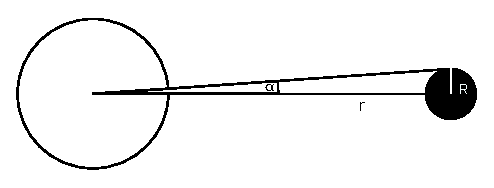
\includegraphics{sketch1.eps}
\end{center}

\begin{align*}
\frac{P_{solar}}{A(r)}=\frac{P_{solar}*}{A*}\\
\Leftrightarrow P_{solar}=\frac{P_{solar}\cdot 4\pi r^2}{A*}
\end{align*}

$A(r)$ is the surface of a radiation sphere with the radius $r$.\\
$A*$, on the other hand, is the surface area equivalent to a sphere with radius $r$ and canonical spacial angle $\Omega$ given by an angle $\alpha$:

\begin{align*}
A*=r^2\Omega \quad \quad \Omega=4\pi\sin^2(\frac{\alpha}{2}) \quad \quad \tan\alpha = \frac{R}{r}
\end{align*}

This leads to:

\begin{equation*}
A*=4\pi r^2\sin^2\left(\frac{\arctan(\frac{R}{r})}{2}\right)
\end{equation*}

Returning to our main equation and inserting the expressions for $A*$ and $P_{solar}$*, we obtain:
\begin{align*}
P_{solar}&=\frac{\sigma 4\pi R^2 T^4 \cdot 4 \pi r^2}{4\pi r^2\sin^2\left(\frac{\arctan(\frac{R}{r})}{2}\right)}\\
&=\frac{\sigma 4\pi R^2 T^4}{\sin^2\left(\frac{\arctan(\frac{R}{r})}{2}\right)}\\
&=\frac{5,670\cdot 10^{-8}Wm^{-2}K^{-4}\cdot 4\pi \cdot 6371^2\cdot 10^6m^2 \cdot 290^4K^4}{\sin^2\left(\frac{\arctan\left(\frac{6371\cdot 10^3}{1,5\cdot 10^{11}}\right)}{2}\right)}\\
&\approx 4,5355\cdot 10^{26}W
\end{align*}

Which roughly coincides with the literature values, the latter ones also having an order of magnitude of 26.

\item $r_{Titan}=1,429\cdot 10^{12}m \quad R_{Titan}=5150\cdot 10^3m$

Using our results from (1), we derive:

\begin{align*}
{T_{Titan}}^4&=\sqrt[4]{\frac{P_{solar} \sin^2\left(\frac{\arctan\left(\frac{R_{Titan}}{r_{Titan}}\right)}{2}\right)}{\sigma 4\pi {R_{Titan}}^2}}\\
&=\sqrt[4]{\frac{4,5355\cdot 10^{26}W\cdot \sin^2\left(\frac{\arctan\left(\frac{5150\cdot 10^3}{1,4294\cdot 10^{12}}\right)}{2}\right)}{5,670\cdot 10^{-8}Wm^{-2}K^{-4}\cdot 4\pi \cdot 5150^2\cdot 10^6m^2}}\\
&\approx 93,94K
\end{align*}

The result coincides almost perfectly with the literature value.

\item $r_{solar}=0,7\cdot 10^9m \quad T_{solar}=5800K \quad m_{solar}=2\cdot 10^{30}kg$

The rest mass is given by:
\begin{equation*}
E_0=m_0c^2
\end{equation*}

The solar loss of rest mass per time can thus be calculated:
\begin{align*}
m_0&=\frac{P_{solar}t}{c^2}\\
\Leftrightarrow \frac{m_0}{t}&=\frac{\sigma 4\pi {r_{solar}}^2{T_{solar}}^4}{c^2}\\
\Leftrightarrow \frac{m_0}{t}&=\frac{5,670\cdot 10^{-8}Wm^{-2}T^{-4}\cdot 4\pi \cdot 0,7^2\cdot 10^{18}m^2 \cdot 5800^4 K^4}{299792458^2m^2s^{-2}}\\
&\approx 4,3960 \cdot 10^{9}kgs^{-1}
\end{align*}

In an entire year, this sums up to a relative loss of:
\begin{align*}
p = \frac{m_0(t)}{m_{solar}} &= \frac{P_{solar}t}{c^2m_{solar}}\\
&=\frac{5,670\cdot 10^{-8}Wm^{-2}T^{-4}\cdot 4\pi \cdot 0,7^2\cdot 10^{18}m^2 \cdot 5800^4 K^4 \cdot 3600\cdot 24\cdot 365s}{299792458^2m^2s^{-2}\cdot 2\cdot 10^{30}kg}\\ 
&\approx 6,9316 \cdot 10^{-14}=6,9316\cdot 10^{-11} %
\end{align*}

\end{enumerate}

\end{document}

